%
% Quantum Repeater Networks
%

\section{Quantum repeater networks} \label{sec:rep_net} \index{Quantum repeater networks}

In the previous Sec.~\ref{sec:ent_ultimate} we concluded that quantum networks specialising purely in entanglement distribution (Bell-pairs in the simplest case), would already be extremely capable in enabling many distributed quantum protocols. This motivates the development of protocols for entanglement distribution over noisy, long-distance quantum networks.

\textit{Quantum repeaters} are devices that allow high-quality entanglement to be shared between distant nodes, when no direct line of communication is available from a server to its two clients. For example, a satellite in low Earth orbit (Sec.~\ref{sec:quant_space_race}) may be outside simultaneous line-of-sight\index{Line-of-sight} to two distinct ground stations\index{Ground stations}, owing simply to the Earth's curvature\index{Earth curvature}. This is achieved using a bootstrapped entanglement swapping and purification protocol (Secs.~\ref{sec:swapping} \& \ref{sec:ent_purif}). Most commonly, this entanglement is in the form of Bell-pairs\index{EPR pairs}, which, as discussed previously in Sec.~\ref{sec:ent_ultimate}, form a ubiquitous resource for many essential quantum protocols. The actual physical encoding of the entangled states may vary, but is most commonly and archetypically in the form of polarisation-encoded\index{Polarisation encoding} single-photons or CV states\index{Continuous-variable states}.

\comment{To do by Bill Munro}

\comment{Update figure PDFs to latest versions from Illustrator}

\comment{Smaller (a), (b) etc.}

\begin{figure}[!htb]
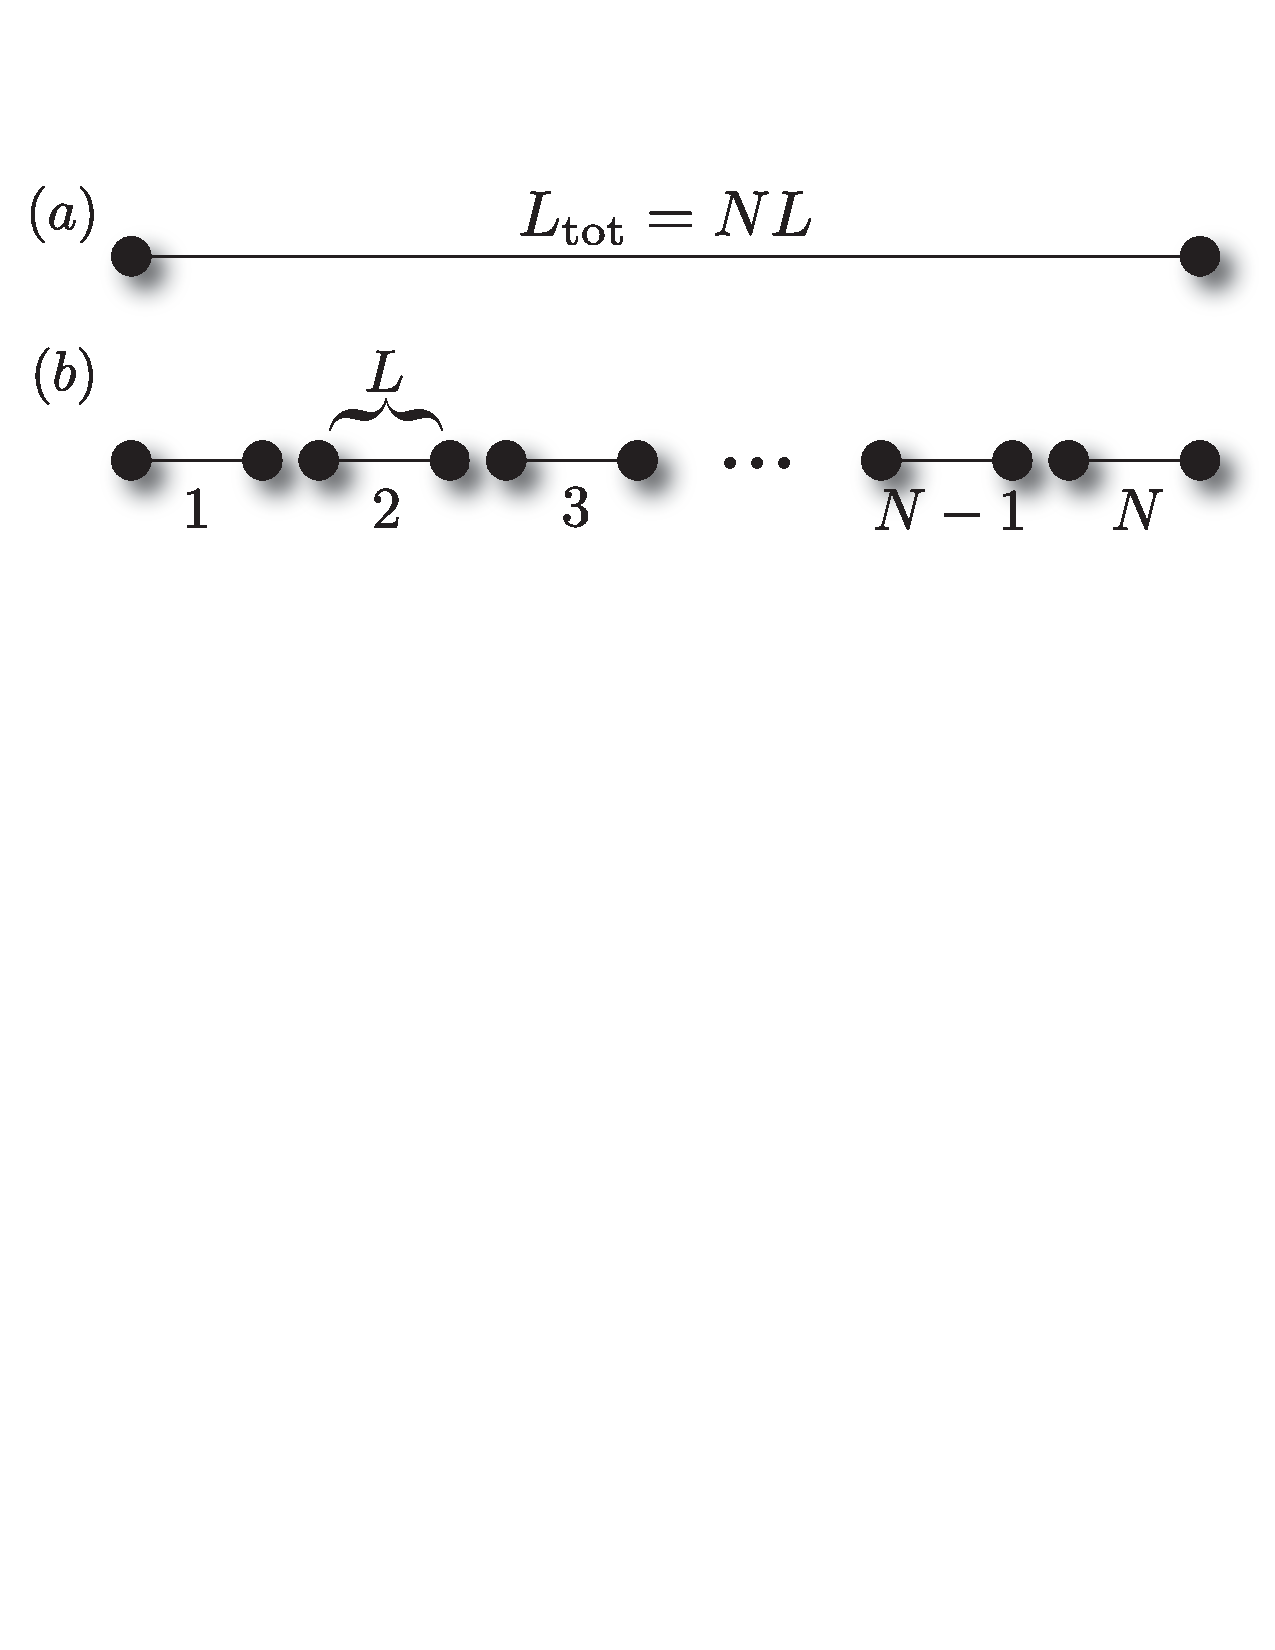
\includegraphics[width=0.47\textwidth]{repeaters_1}
\caption{} \label{fig:repeaters_1}	
\end{figure}

\begin{figure}[!htb]
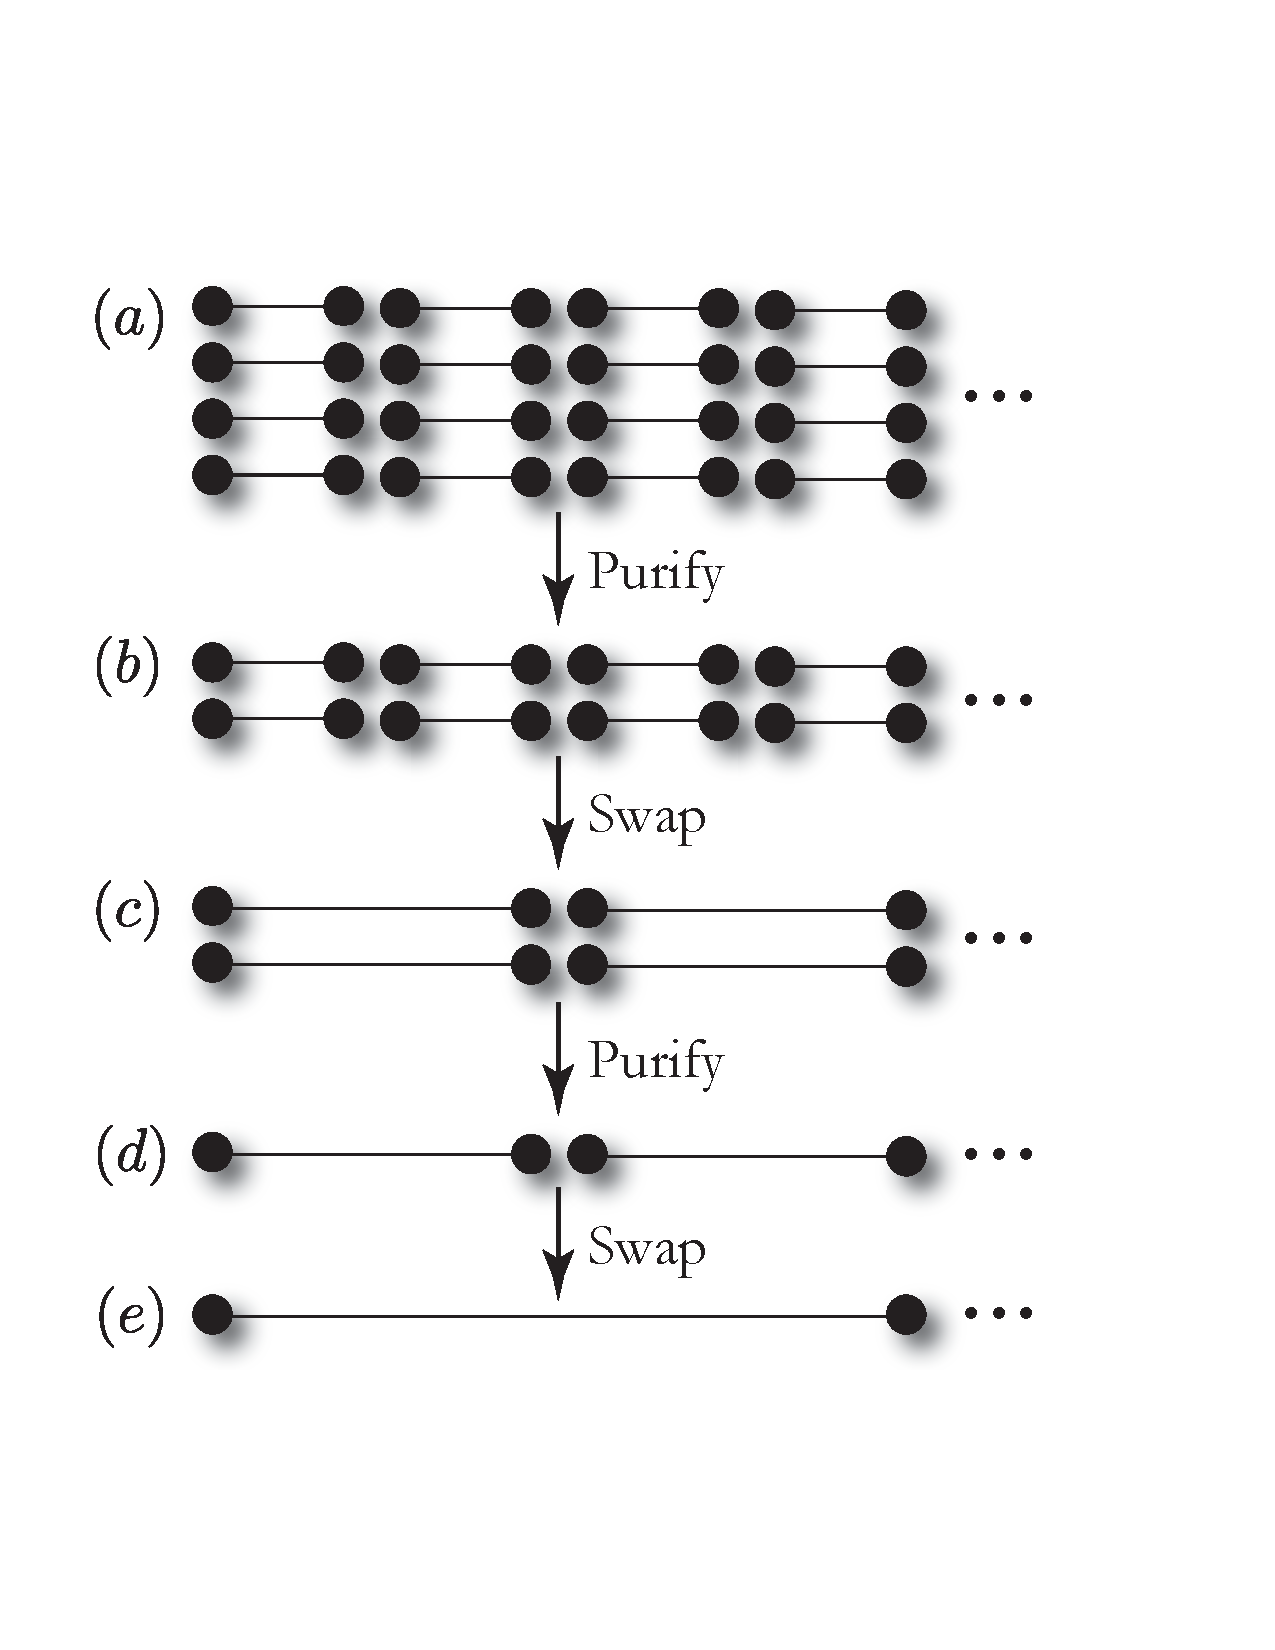
\includegraphics[width=0.47\textwidth]{repeaters_2}
\caption{} \label{fig:repeaters_2}	
\end{figure}

\begin{figure}[!htb]
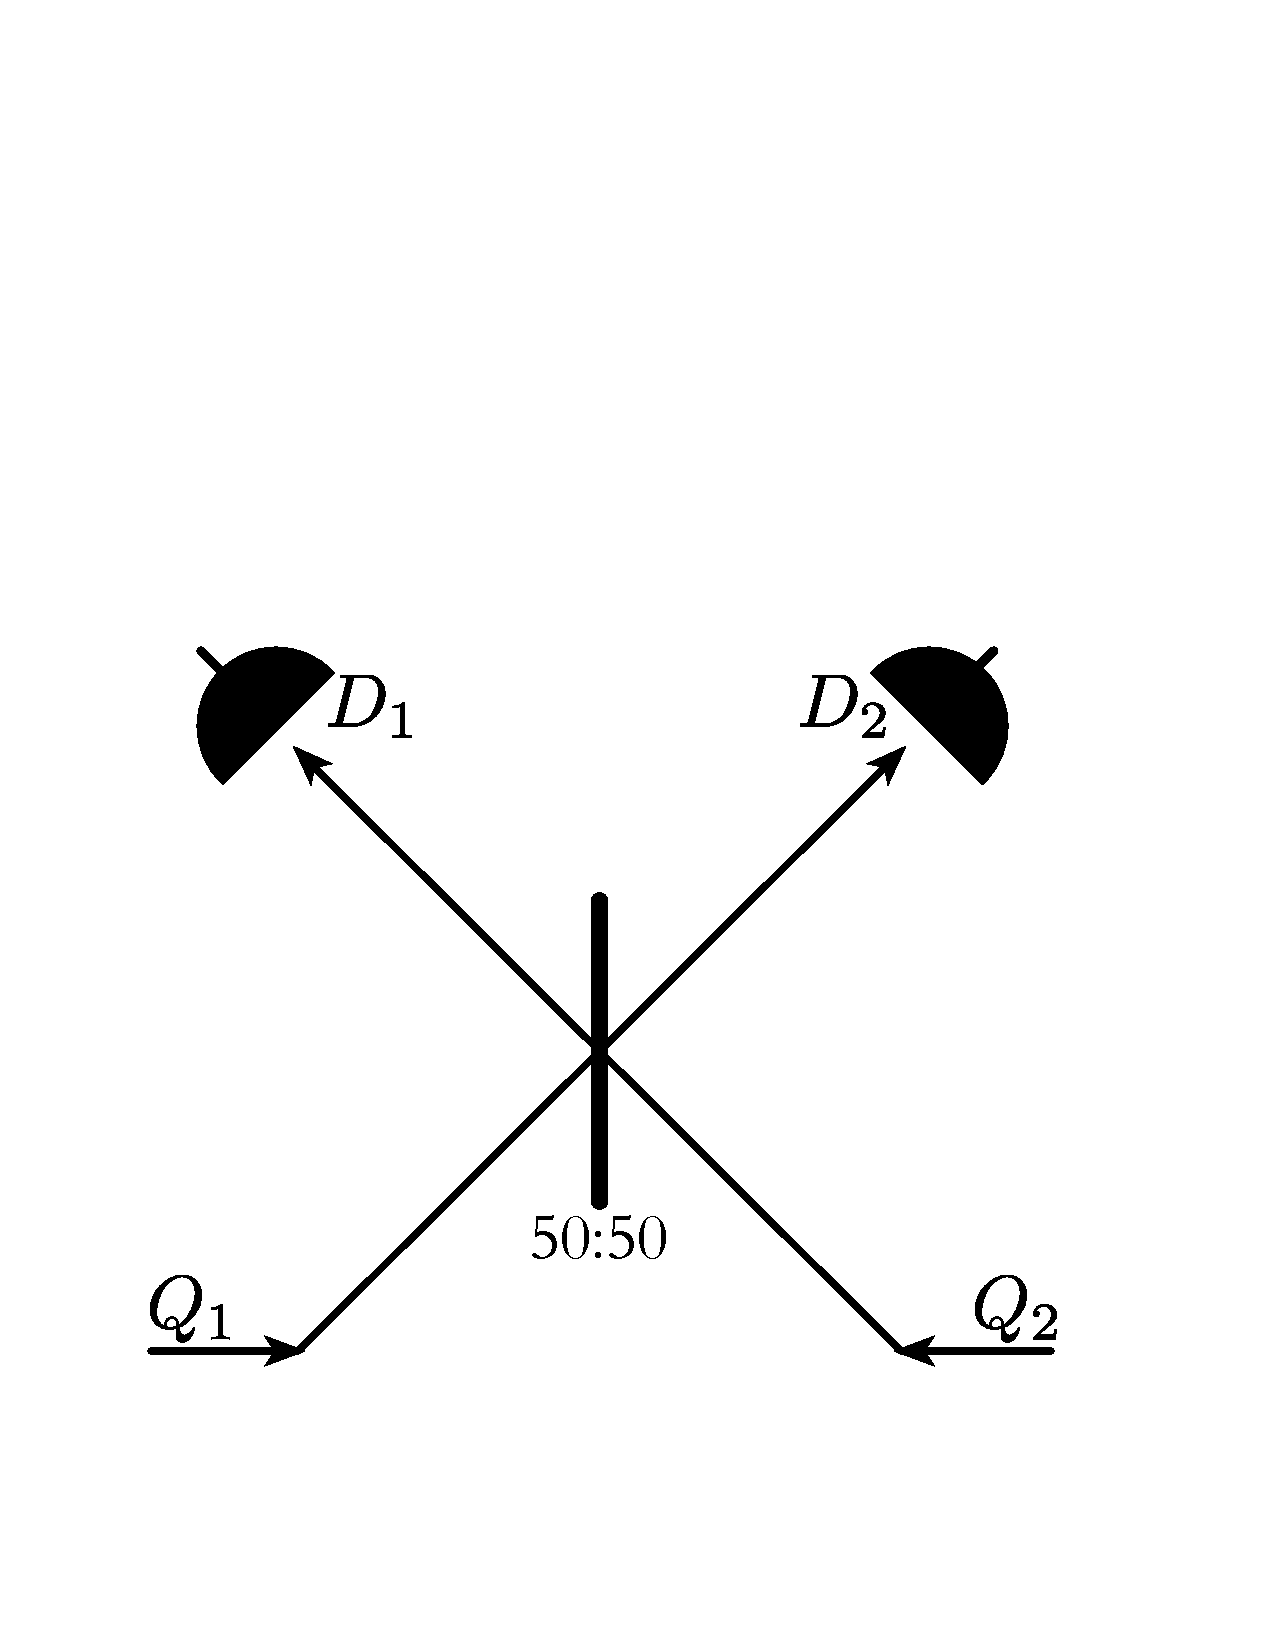
\includegraphics[width=0.47\textwidth]{repeaters_3}
\caption{} \label{fig:repeaters_3}	
\end{figure}

\begin{figure}[!htb]
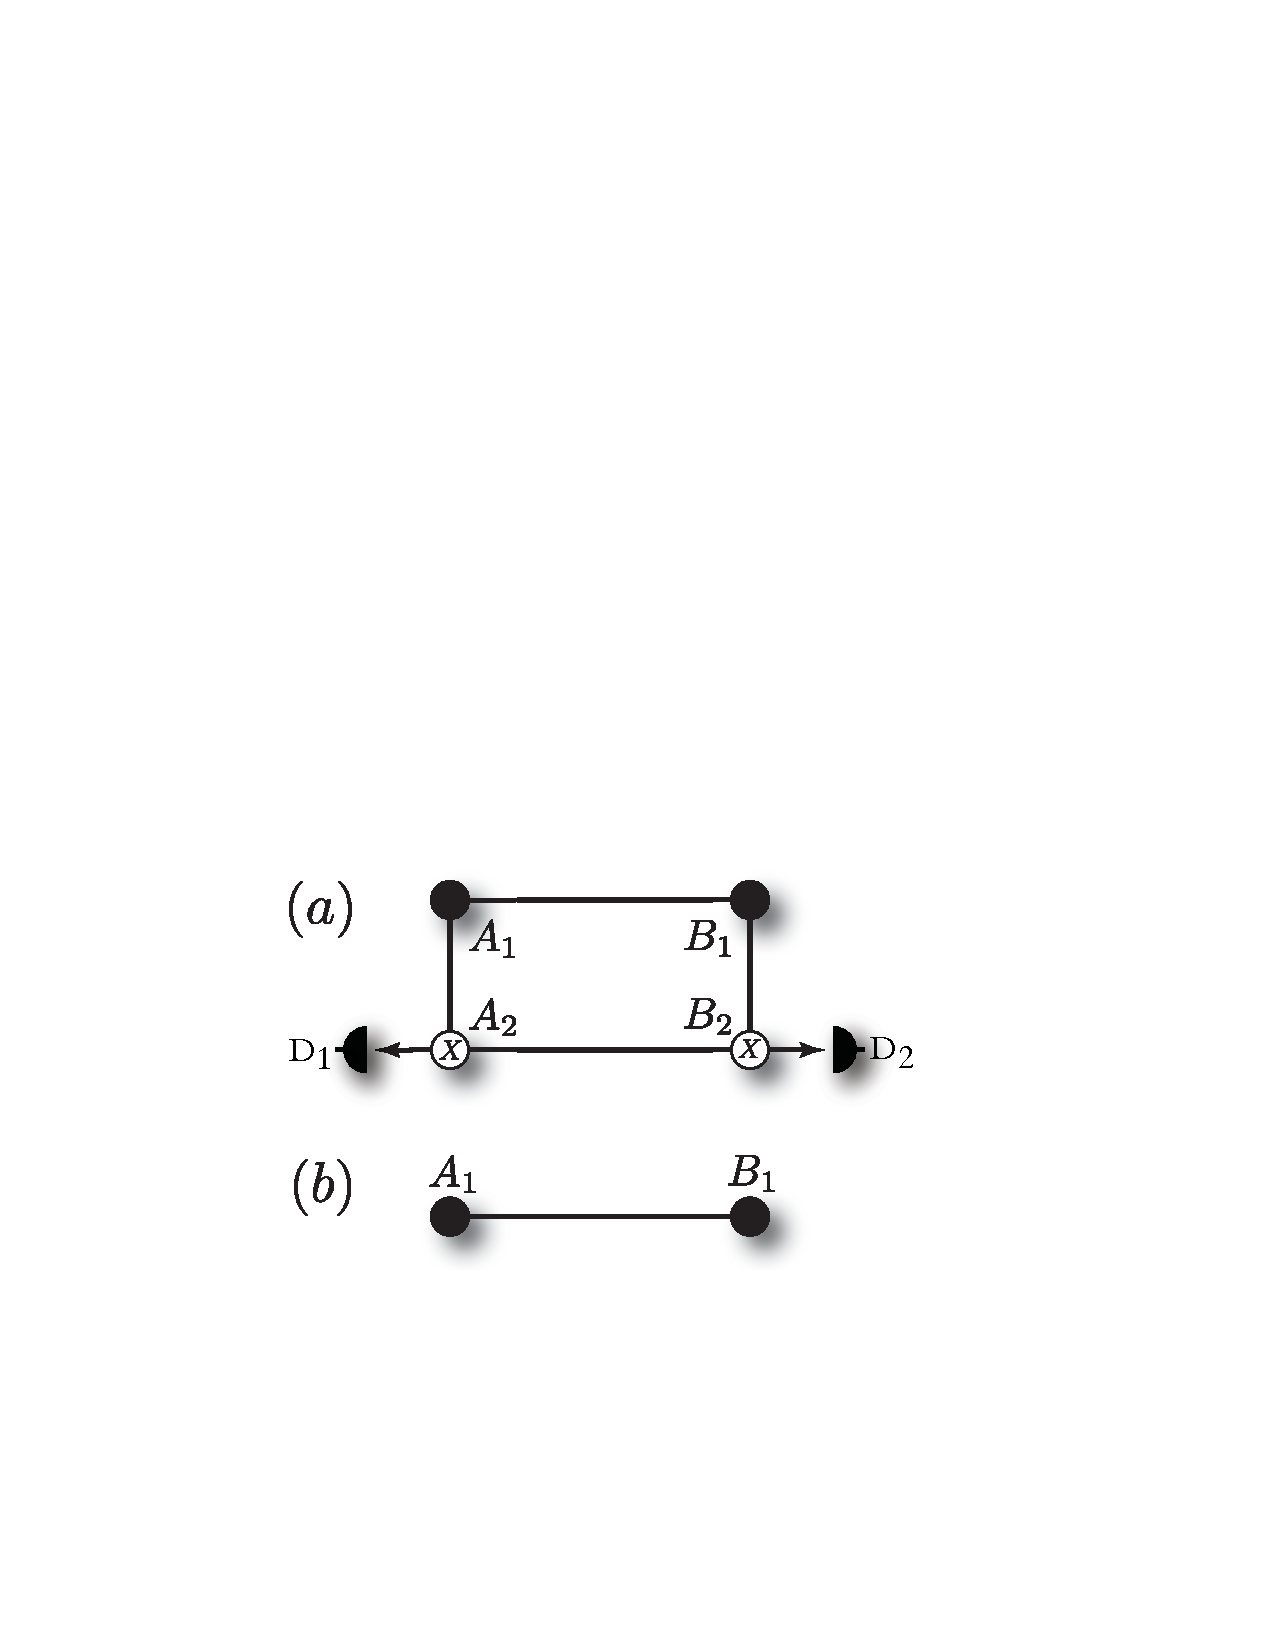
\includegraphics[width=0.47\textwidth]{repeaters_4}
\caption{} \label{fig:repeaters_4}	
\end{figure}

\begin{figure}[!htb]
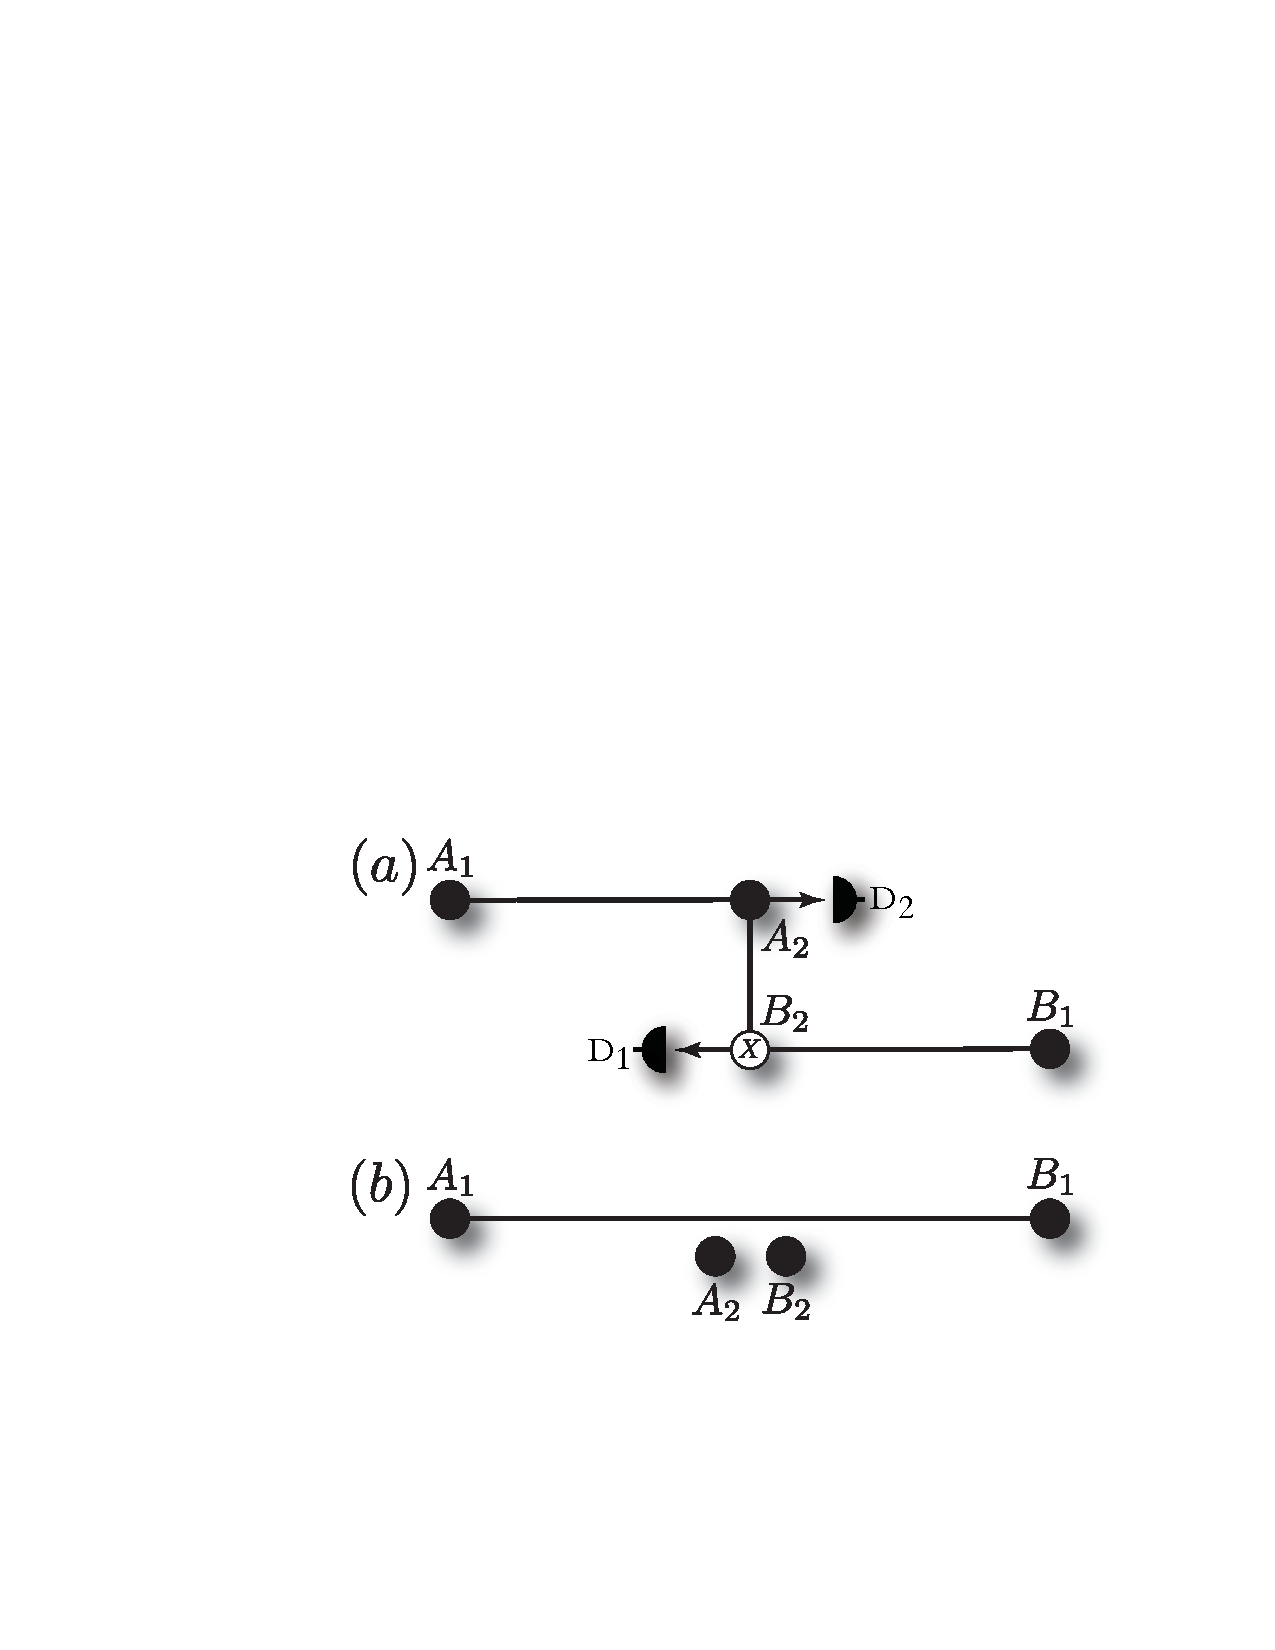
\includegraphics[width=0.47\textwidth]{repeaters_5}
\caption{} \label{fig:repeaters_5}
\end{figure}

\comment{Latin quote}\index{Latin}